\documentclass[a4paper,11pt]{article}

\usepackage[english]{babel}
\usepackage{float}
\usepackage{graphicx}
\usepackage{amsmath,amsthm}
\usepackage{gensymb}
\usepackage{amssymb}
\usepackage[margin=2.cm]{geometry}
\usepackage{pstricks-add}	%for geometric diagrams
\usepackage{chemfig}	%for structural formulae
\usepackage{tabularx}	%for better tables
\usepackage{booktabs}	%for better tables
\usepackage[makeroom]{cancel}	%for cancelling lines
\usepackage{hyperref}	%hyperlinks
\usepackage{mathrsfs}
\usepackage{mathtools}
\usepackage{epigraph}	%quotes
\usepackage{lastpage}
\usepackage{multicol}	%column environments
\usepackage{fancyhdr}	%headers
\usepackage[at]{easylist}	%easy lists
\usepackage{wasysym}
\usepackage{wrapfig}	%wrap figures in text
\usepackage{subfig}		%subfigures
\usepackage{tikz}

\allowdisplaybreaks
\newcommand\numberthis{\addtocounter{equation}{1}\tag{\theequation}}
\setlength{\epigraphwidth}{7.7cm}
\setlength{\tabcolsep}{10pt}

% bracket group shorthands
\newcommand{\abs}[1]{\left|#1\right|}
\newcommand{\set}[1]{\left\{#1\right\}}

% common sets
\newcommand{\R}{\mathbb{R}}
\newcommand{\Cmplx}{\mathbb{C}}
\newcommand{\Q}{\mathbb{Q}}
\newcommand{\Z}{\mathbb{Z}}
\newcommand{\N}{\mathbb{N}}

% derivative shorthands
\newcommand{\diff}[2]{\frac{\mathrm{d}#1}{\mathrm{d}#2}}
\newcommand{\pdiff}[2]{\frac{\partial #1}{\partial #2}}
\newcommand{\ndiff}[3]{\frac{\mathrm{d}^{#3}#1}{\mathrm{d}#2^{#3}}}
\newcommand{\npdiff}[3]{\frac{\partial^{#3} #1}{\partial #2^{#3}}}

% theorem environments
\newtheorem*{definition*}{Definition}
\newtheorem*{lemma*}{Lemma}
\newtheorem{theorem}{Theorem}
\newtheorem*{theorem*}{Theorem}
\newtheorem*{corollary*}{Corollary}
\newtheorem{example}{Example}
\newtheorem*{remark}{Remark}

\DeclareMathOperator{\bdy}{Bdy}
\DeclareMathOperator{\interior}{Int}

% header
\pagestyle{fancy}
\lhead{Question Breakdown - Set 1, Question 8}
\rhead{Year 11 2018}

%\title{Question Breakdown - Set 1, Question 8}
%\date{\today}
%\author{Daniel Czapski}

\begin{document}
	\section*{Question Breakdown - Set 1, Question 8}
\begin{center}
	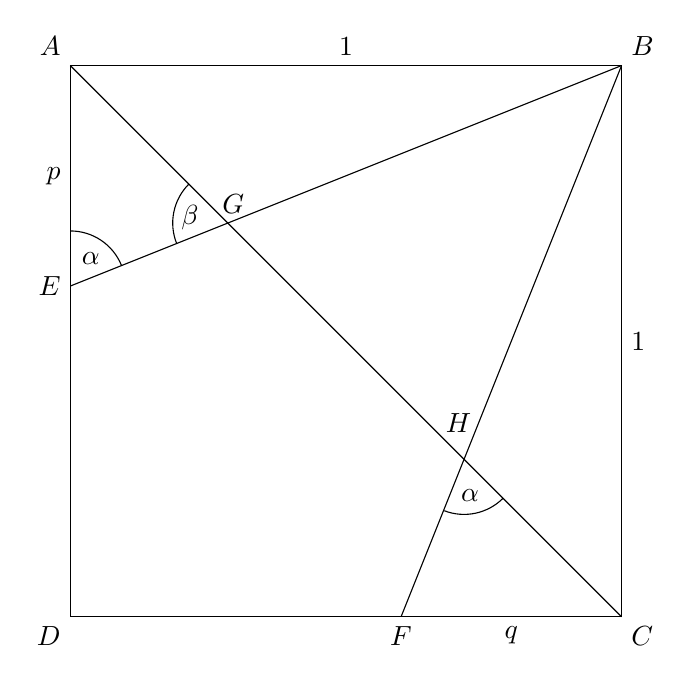
\begin{tikzpicture}[scale=7]
	\draw (0,0) rectangle (1,1);
	\draw (0,1) -- (1,0);
	\draw (0,0.6) -- (1,1);
	\draw (0.6,0) -- (1,1);
	
	\draw (0,0.7) arc (90:22:0.1);
	\draw (0.214989,0.785011) arc (135:202:0.1);
	\draw (0.785011,0.214989) arc (-45:-111:0.1);
	
	\node[above left] at (0,1) {$A$};
	\node[left] at (0,0.8) {$p$};
	\node[left] at (0,0.6) {$E$};
	\node[below left] at (0,0) {$D$};
	\node[below] at (0.6,0) {$F$};
	\node[below] at (0.8,0) {$q$};
	\node[below right] at (1,0) {$C$};
	\node[right] at (1,0.5) {$1$};
	\node[above right] at (1,1) {$B$};
	\node[above] at (0.5,1) {$1$};
	\node[above] at (0.2957,0.7143) {$G$};
	\node[above] at (0.7043,0.3157) {$H$};
	
	\node at (0.037,0.65) {$\alpha$};
	\node at (0.217,0.724) {$\beta$};
	\node at (0.725,0.22) {$\alpha$};
	\end{tikzpicture}
\end{center}
In the diagram, $ABCD$ is a unit square. Points $E$ and $F$ are chosen on $AD$ and $DC$ respectively, such that $\angle AEG=\angle FHC$, where $G$ and $H$ are the points at which $BE$ and $BF$ respectively cut the diagonal $AC$.\\

\noindent Let $AE=p$, $FC=q$, $\angle AEG=\alpha$ and $\angle ABE=\beta$.
\vspace{0.15cm}

\begin{easylist}
	\ListProperties(Start1=1,Numbers1=r,Margin=1cm,FinalMark1={)},Space*=0.5cm)
	@ Express $\alpha$ in terms of $p$ and $\beta$ in terms of $q$. (2 marks)
	@ Prove that $p+q=1-pq$. (2 marks)
	@ Show that the area of the quadrilateral $EBFD$ is given by
	$$
	1-\frac{p}{2}+\frac{p-1}{2(p+1)}.\quad \text{(1 mark)}
	$$
	@ What is the maximum value of the area of $EBFD$? (2 marks)\\
\end{easylist}
\vspace{0.15cm}

\noindent This question is a more difficult application of plane geometry and right-angled trigonometry. The first two parts of the question are probably the most difficult, but the question is constructed such that one can at least do parts iii and iv if parts i and ii prove too difficult.

\begin{remark}\normalfont
This is quite common. More difficult questions will often be written such that subsequent parts depend on previous parts, but if one is unable to do the previous part, the result can still be used, and some marks can still be attained. This is particularly common in questions such as this one where one is required to prove a particular result. Even if the proof is not completed, one can take the result as given for the rest of the question. 
\end{remark}

\noindent The best place to start in a trigonometric or geometric problem such as this is with a diagram. It's usually a good idea to copy down the diagram given in the question (if one is given). In particular, ensure that your diagram 
\vspace{0.15cm}
\begin{easylist}[itemize]
@ is \textbf{large} (about half a page is sufficient);
@ \textbf{contains all the information given} in the question (in this case, the angles at $A$, $B$ and $C$);
@ \textbf{contains what you are required to find} (the bearing of $B$ from Uluru, which will involve the angle between $B$ and North);
@ if necessary, \textbf{contains other quantities that you define}; and
@ has \textbf{North labelled clearly} (if the question involves bearings).\\
\end{easylist}

\begin{remark}\normalfont 
Once you draw a diagram, read through the question again to ensure that all information given is present. Often, diagrams given in the question will lack at least one piece of information which is usually crucial to the problem to make sure you're actually reading the question.
\end{remark}

i) For part i, we first examine $\triangle ABE$. In particular, we can write that
\begin{align*}
\tan(\alpha) &= \dfrac{1}{p}\\
\implies \alpha &= \tan^{-1}\left(\frac{1}{p}\right). \footnote{There is some subtlety to this but it is beyond the scope of the year 11 course.}
\end{align*}
That was the easy bit. We would very much like to do something similar for $\beta$ and $q$ in $\triangle BCF$, however $\angle HFC$ is currently unknown. We note that $\angle EAG = \angle FCH = 45\degree$, since $ABCD$ is a square, $AC$ is a diagonal and diagonals bisect interior angles they pass through in rhombuses (of which squares are a subset). We should put this on our diagram.

\begin{center}
	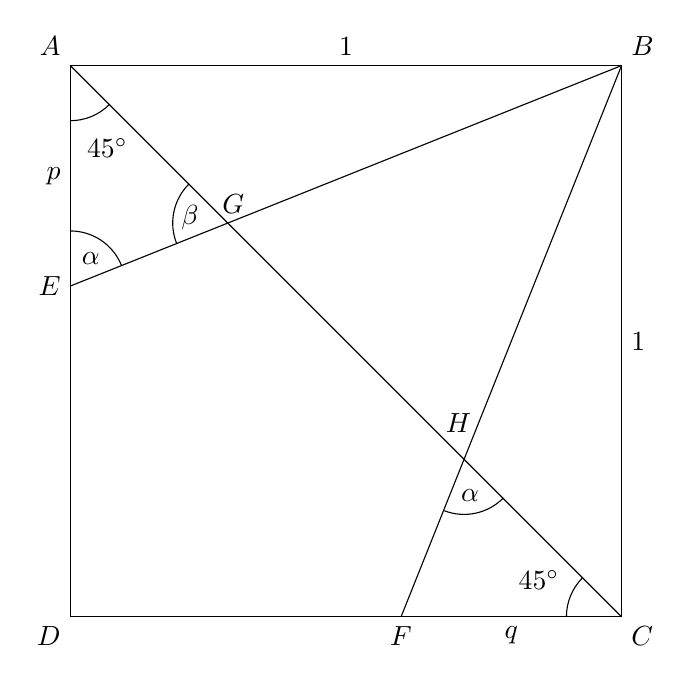
\begin{tikzpicture}[scale=7]
	\draw (0,0) rectangle (1,1);
	\draw (0,1) -- (1,0);
	\draw (0,0.6) -- (1,1);
	\draw (0.6,0) -- (1,1);
	
	\draw (0,0.7) arc (90:22:0.1);
	\draw (0.214989,0.785011) arc (135:202:0.1);
	\draw (0.785011,0.214989) arc (-45:-111:0.1);
    
    \draw (0,0.9) arc (-90:-45:0.1);
    \draw (0.9,0) arc (180: 135:0.1);
	
	\node[above left] at (0,1) {$A$};
	\node[left] at (0,0.8) {$p$};
	\node[left] at (0,0.6) {$E$};
	\node[below left] at (0,0) {$D$};
	\node[below] at (0.6,0) {$F$};
	\node[below] at (0.8,0) {$q$};
	\node[below right] at (1,0) {$C$};
	\node[right] at (1,0.5) {$1$};
	\node[above right] at (1,1) {$B$};
	\node[above] at (0.5,1) {$1$};
	\node[above] at (0.2957,0.7143) {$G$};
	\node[above] at (0.7043,0.3157) {$H$};
	
	\node at (0.037,0.65) {$\alpha$};
	\node at (0.217,0.724) {$\beta$};
	\node at (0.725,0.22) {$\alpha$};
    
    \node at (0.067,0.85) {$45\degree$};
    \node at (0.85,0.067) {$45\degree$};
	\end{tikzpicture}
\end{center}

\noindent Now, looking at triangles $AEG$ and $CFH$, we have that
\begin{align*}
\angle EAG = \angle FCH && \angle AEG = \angle FHC.
\end{align*}
Thus, we may conclude $\triangle AEG\ |||\ \triangle FHC$. Since corresponding angles in similar triangles are equal, we must have that $\angle CFH = \beta$. We will put this on our diagram as well.

\begin{center}
	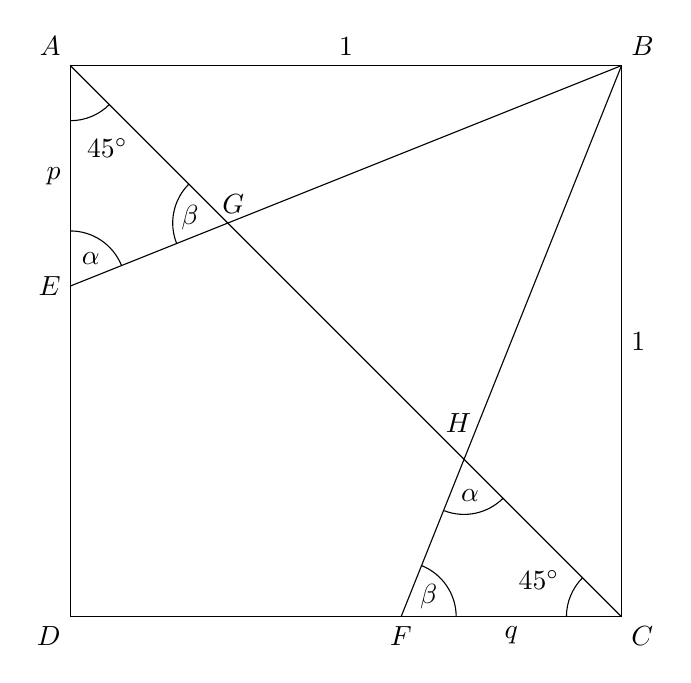
\begin{tikzpicture}[scale=7]
	\draw (0,0) rectangle (1,1);
	\draw (0,1) -- (1,0);
	\draw (0,0.6) -- (1,1);
	\draw (0.6,0) -- (1,1);
	
	\draw (0,0.7) arc (90:22:0.1);
	\draw (0.214989,0.785011) arc (135:202:0.1);
	\draw (0.785011,0.214989) arc (-45:-111:0.1);
	\draw (0.7,0) arc (0:68:0.1);
    
    \draw (0,0.9) arc (-90:-45:0.1);
    \draw (0.9,0) arc (180: 135:0.1);
	
	\node[above left] at (0,1) {$A$};
	\node[left] at (0,0.8) {$p$};
	\node[left] at (0,0.6) {$E$};
	\node[below left] at (0,0) {$D$};
	\node[below] at (0.6,0) {$F$};
	\node[below] at (0.8,0) {$q$};
	\node[below right] at (1,0) {$C$};
	\node[right] at (1,0.5) {$1$};
	\node[above right] at (1,1) {$B$};
	\node[above] at (0.5,1) {$1$};
	\node[above] at (0.2957,0.7143) {$G$};
	\node[above] at (0.7043,0.3157) {$H$};
	
	\node at (0.037,0.65) {$\alpha$};
	\node at (0.217,0.724) {$\beta$};
	\node at (0.725,0.22) {$\alpha$};
	\node at (0.65,0.037) {$\beta$};
    
    \node at (0.067,0.85) {$45\degree$};
    \node at (0.85,0.067) {$45\degree$};
	\end{tikzpicture}
\end{center}

Now that we have the angle $BFC$, we can write 
\begin{align*}
\tan(\beta) &= \frac{1}{q}\\
\implies \beta &= \tan^{-1}\left(\frac{1}{q}\right).
\end{align*}
So, overall, we have
\begin{align*}
\tan(\alpha) &= \frac{1}{p} && \tan(\beta) = \frac{1}{q}
\end{align*}
or
\begin{align*}
\alpha &= \tan^{-1}\left(\frac{1}{p}\right) && \beta = \tan^{-1}\left(\frac{1}{q}\right).
\end{align*}\\

ii) We are required to prove 
$$
p+q = 1-pq.
$$
From the previous part, we have that 
\begin{align*}
p+q &= \frac{1}{\tan(\alpha)} + \frac{1}{\tan(\beta)}\\
&= \frac{\tan(\alpha) + \tan(\beta)}{\tan(\alpha)\tan(\beta)}.\numberthis\label{pq1}
\end{align*}
Additionally, 
\begin{align*}
1-pq &= 1-\frac{1}{\tan(\alpha)\tan(\beta)}\\
&= \frac{\tan(\alpha)\tan(\beta)-1}{\tan(\alpha)\tan(\beta)}.\numberthis\label{pq2}
\end{align*}
Dividing equation (\ref{pq1}) by (\ref{pq2}), we obtain
\begin{align*}
\frac{p+q}{1-pq} &= \frac{\tan(\alpha) + \tan(\beta)}{\tan(\alpha)\tan(\beta)}\frac{\tan(\alpha)\tan(\beta)}{\tan(\alpha)\tan(\beta)-1}\\
&= \frac{\tan(\alpha)+\tan(\beta)}{\tan(\alpha)\tan(\beta)-1}\\
&=-\tan(\alpha+\beta).\numberthis\label{pq3}
\end{align*}
\pagebreak

\noindent Now, examining either $\triangle AEG$ or $\triangle CFH$, the angle sum of a triangle requires that
$$
\alpha+\beta+45\degree = 180\degree \iff \alpha+\beta = 135\degree.
$$
Thus, taking the tan of both sides,
\begin{align*}
\tan(\alpha+\beta) &= \tan(135\degree)\\
&= -1.\numberthis\label{pq4}
\end{align*}
Substituting this result into equation (\ref{pq3}), we see that
\begin{align*}
\frac{p+q}{1-pq} &= -\tan(\alpha+\beta)\\
&= -(-1)\\
&= 1.\\
\iff p+q &= 1-pq \numberthis\label{pq5}
\end{align*}
as required.\\

iii) We are required to show that the area of the quadrilateral $EBFD$ is given by
$$
1-\frac{p}{2}+\frac{p-1}{2(p+1)}.
$$
We refer back to our diagram.
\begin{center}
	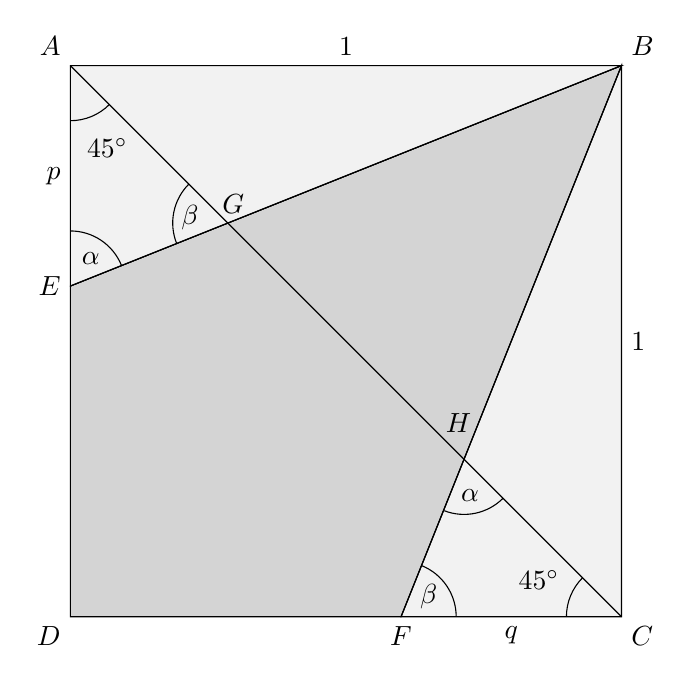
\begin{tikzpicture}[scale=7]
    %\draw[fill=lightgray] (0,0.6) -- (0,0) -- (0.6,0) -- (1,1) -- cycle;
    \draw[fill={rgb:lightgray,2;white,1}] (0,0.6) -- (0,0) -- (0.6,0) -- (1,1) -- cycle;
    \draw[fill={rgb:lightgray,1;white,4}] (0,0.6) -- (0,1) -- (1,1) -- cycle;
    \draw[fill={rgb:lightgray,1;white,4}] (0.6,0) -- (1,1) -- (1,0) -- cycle;
    
	\draw (0,0) rectangle (1,1);
	\draw (0,1) -- (1,0);
	\draw (0,0.6) -- (1,1);
	\draw (0.6,0) -- (1,1);
	
	\draw (0,0.7) arc (90:22:0.1);
	\draw (0.214989,0.785011) arc (135:202:0.1);
	\draw (0.785011,0.214989) arc (-45:-111:0.1);
	\draw (0.7,0) arc (0:68:0.1);
    
    \draw (0,0.9) arc (-90:-45:0.1);
    \draw (0.9,0) arc (180: 135:0.1);
	
	\node[above left] at (0,1) {$A$};
	\node[left] at (0,0.8) {$p$};
	\node[left] at (0,0.6) {$E$};
	\node[below left] at (0,0) {$D$};
	\node[below] at (0.6,0) {$F$};
	\node[below] at (0.8,0) {$q$};
	\node[below right] at (1,0) {$C$};
	\node[right] at (1,0.5) {$1$};
	\node[above right] at (1,1) {$B$};
	\node[above] at (0.5,1) {$1$};
	\node[above] at (0.2957,0.7143) {$G$};
	\node[above] at (0.7043,0.3157) {$H$};
	
	\node at (0.037,0.65) {$\alpha$};
	\node at (0.217,0.724) {$\beta$};
	\node at (0.725,0.22) {$\alpha$};
	\node at (0.65,0.037) {$\beta$};
    
    \node at (0.067,0.85) {$45\degree$};
    \node at (0.85,0.067) {$45\degree$};
    
	\end{tikzpicture}
\end{center}
It is clear that the area of the quadrilateral $EBFD$ (the darker area) is the area of the square less the areas of triangles $AEB$ and $CFH$ (the lighter areas). Let $A$ be the area of the quadrilateral required, and $A_s$, $A_p$ and $A_q$ be the areas of the square and the two triangles hitherto referenced respectively. Then, 
\begin{align*}
A &= A_s - A_q - A_q.
\end{align*}
Now, we are given that the square $ABCD$ is a unit square, so $A_s=1$. Recalling that the area of a triangle is given by $A=\frac{1}{2}bh$ where $b$ and $h$ are the base length and perpendicular height respectively, we see that
\begin{align*}
A_p = \frac{p}{2} && A_q = \frac{q}{2}.
\end{align*}
So, 
\begin{align*}
A = 1 - \frac{p}{2} - \frac{q}{2}.\numberthis\label{a1}
\end{align*}
\pagebreak

\noindent Now, recall from part ii we have equation (\ref{pq5}). We note that the expression we are required to obtain involves only $p$, so we can use this previous result to eliminate $q$. In particular, 
\begin{align*}
p+q &= 1-pq\\
\iff q(1+p) &= 1-p\\
\iff q &= \frac{1-p}{1+p}.\numberthis\label{a2}
\end{align*}
Substituting equation (\ref{a2}) into equation (\ref{a1}), we have that
\begin{align*}
A &= 1 - \frac{p}{2} -\frac{1-p}{2(1+p)}\\
&= 1 - \frac{p}{2} +\frac{p-1}{2(p+1)}
\end{align*}
as required.\\

iv) The last part of the question mandates that we maximise the area found in the previous question. That is, we wish to maximise
\begin{align*}
A = 1 - \frac{p}{2} +\frac{p-1}{2(p+1)}.\numberthis\label{a3}
\end{align*}
We note initially
\begin{align*}
\diff{A}{p} &= \diff{}{p}\left(1 - \frac{p}{2} + \frac{p-1}{2(p+1)}\right)\\
&= -\frac{1}{2} + \frac{p+1-(p-1)}{2(p+1)^2}\\
&= \frac{1}{(p+1)^2}-\frac{1}{2}
\end{align*}
through judicious application of the appropriate differentiation theorems. To determine the values of $p$ for which extrema occur, we solve the equation $\diff{A}{p} = 0$. That is,
\begin{align*}
\frac{1}{(p+1)^2}-\frac{1}{2} &= 0\\
(p+1)^2 &= 2\\
p+1 &= \sqrt{2}\\
p &= \sqrt{2}-1
\end{align*}
where the third line follows from the fact that $p$ is a distance, so $p>0$, thus $p+1>0$.\\

\noindent In order to determine whether this is a local maximum or minimum, we check the value of the second derivative. We have that
\begin{align*}
\diff{A}{p} &= (p+1)^{-2}-\frac{1}{2}\\
\implies \ndiff{A}{p}{2} &= -\frac{2}{(p+1)^3} < 0 \text{ for all }p>0.
\end{align*}
Since the second derivative is negative for all $p$, thus for $p=\sqrt{2}-1$, we have a local maximum at $p=\sqrt{2}-1$, as we expect.
\begin{remark}\normalfont
Do not forget to determine the nature of the stationary point! The fact that the question tells you that you're supposed to find a maximum is not a sufficiently rigorous reason to state a point is a local maximum without further justification.
\end{remark}
\noindent The question requests we determine the maximal area, so we substitute $p=\sqrt{2}-1$ into equation (\ref{a3}) and simplify. We acquire
\begin{align*}
A_{\text{max}} &= 1 - \frac{\sqrt{2}-1}{2} +\frac{\sqrt{2}-1-1}{2(\sqrt{2}-1+1)}\\
&= 1 - \frac{\sqrt{2}-1}{2} + \frac{\sqrt{2}-2}{2\sqrt{2}}\\
&= \frac{2\sqrt{2}-2+\sqrt{2}+\sqrt{2}-2}{2\sqrt{2}}\\
&= \frac{4\sqrt{2}-4}{2\sqrt{2}}\\
&= 2-\sqrt{2}
\end{align*}
as required.

\vspace{2cm}

If you desire formal tutoring in Preliminary or HSC English, two, three or four units of Mathematics, Science or Economics, Talent 100 offers a comprehensive, structured course taught by a combination of the top HSC achievers of past years, qualified and experienced teachers and leading textbook authors. For HSC success, simplified, contact us on 1300 999 100, check out our website at \url{https://talent-100.com.au/} and find us on Facebook. 

\vfill

\begin{figure}[H]
\centering
\includegraphics[width=0.17\textwidth]{t100.png}
\end{figure}

\end{document}